\documentclass[../../../../main.tex]{subfiles}

\begin{document}

\section*{第1問}

\begin{proof}[解]
$a_n=19^n+(-1)^{n-1}2^{4n-3}$の全てを割り切る数$b$は，$a_1=21,\ a_2=329$の両方を割り切ることが必要で，$b\in\text{prime}$とあわせて，$b=7$が必要。以下，任意の$a_n$が7で割り切れることを示す。

法を7として
\[
a_n\equiv5^n+2(-16)^{n-1}\equiv(-2)^n+(-2)^{n-1}\cdot2\equiv0
\]
より示された。以上から$7$
\end{proof}

\newpage

\section*{第2問}

\begin{proof}[解]
$E(t,-1-t,0)$，$F(u,u,-2u+2)$（$t,u\in\mathbb{R}$とおく）。正四面体の性質上から，$EF$は$\ell_1,\ell_2$と垂直である。
\[
\overrightarrow{EF}=\begin{pmatrix}u-t\\u+t+1\\-2u+2\end{pmatrix}
\]
だから
\[
\overrightarrow{EF}\cdot\begin{pmatrix}-1\\1\\0\end{pmatrix}=0, \qquad
\overrightarrow{EF}\cdot\begin{pmatrix}1\\1\\-2\end{pmatrix}=0
\]
\[
\begin{cases}
(u-t)-(u+t+1)=0 \\
(u-t)+(u+t+1)+4(u-1)=0
\end{cases}
\]
\[
\begin{cases}
t=-\dfrac12 \\
u=\dfrac12
\end{cases}
\]
となり，
\[
E\left(-\frac12,-\frac12,0\right), \qquad F\left(\frac12,\frac12,1\right)
\]

\textbf{(2)} 1辺の長さを$d$とすると，正四面体の面（正三角形）の中線の長さから$BF=\dfrac{\sqrt3}{2}d$。だから$\triangle FEB$にピタゴラスを用いて，
\[
\left(\frac{\sqrt3}{2}d\right)^2=\overline{EF}^2+\left(\frac{d}{2}\right)^2
\]
\[
\overline{EF}=\frac{\sqrt2}{2}d \quad(\because d,\overline{EF}>0)
\]
一方，(1)から$\overline{EF}=\sqrt3$だから，
\[
d=\sqrt6
\]

\textbf{(3)} $A(p,-1-p,0)$とおくと，
\[
\overline{AF}=\sqrt{\left(p-\frac12\right)^2+\left(-p-\frac32\right)^2+1}=\sqrt{2p^2+2p+\frac72}
\]
ここで，(2)から$\overline{AF}=\dfrac{\sqrt3}{2}d=\dfrac32\sqrt2$だから，といて
\[
p=\frac12(-1\pm\sqrt3)
\]
題意から複号正に対応するのが$A$で，
\[
A\left(\frac{-1+\sqrt3}{2},\frac{-1-\sqrt3}{2},0\right)
\]
\end{proof}

\newpage

\section*{第3問}

\begin{proof}[解]
\[
f(x)>0\ (0\le x\le1), \qquad f(0)=2,\ f(1)=1 \quad\cdots\text{①}
\]
又，題意及び①から$k\in\mathbb{R}_{>0}$として，
\[
(x-a)\{f(a)+f(x)\}=k\int_a^xf(t)dt \quad\cdots\text{②}
\]
が$0\le a\le x\le1$なる任意の$a,x$で成立。（$a=x$でも明らかに成立。）$x$で微分して，
\[
f(a)+f(x)+xf'(x)-af'(x)=kf(x)
\]
$y=f(x)$とおく。$a=x=1$として①から$k=2$。次に$a=0$として
\[
2+y+x\frac{dy}{dx}=2y
\]
$y\ne2,\ x\ne0$の時
\[
\frac{dy}{y-2}=\frac{dx}{x} \quad\cdots\text{③}
\]
積分して，
\[
\log|y-2|=\log x+C_1 \quad\cdots\text{④}
\]
ただし，$C_1$は定数。$x=1$は①より，$x\ne0,\ y\ne2$をみたすので，$x=1$で④が成立することから$C_1=0$。したがって
\[
x=|y-2|
\]
したがって，$(x,y)=(1,1)$とあわせて
\[
y=-x+2
\]
これは$x=0$でも成立する。
\end{proof}

\newpage

\section*{第4問}

\begin{proof}[解]
$q=p(p^2-3)$とかける。又，
\[
f(x)=-(x-p)^2+p(p^2-3), \qquad g(x)=x(x^2-3)
\]
とおくと$f(x)=g(x)$の異なる実解が2つである。
\[
g(x)-f(x)=x^3-3x+x^2-2px+p^2-p^3+3p
\]
\[
=(x-p)\left(x^2+(p+1)x+(p^2-p-3)\right)
\]
$\sim$部を$h(x)$とかくと，したがって，$h(x)=0$が$x\ne p$にただ1つ実解を持つ

\textbf{⑦ $h(x)=0$が$x\ne p$に重解を持つ時}

判別式$D$として，
\[
D=-3p^2+6p+13
\]
だから，$D=0\iff p=\dfrac{3\pm4\sqrt3}{3}$の時，だがこれは$0<p<2$に反し不適

\textbf{⑦ $h(x)=0$が$x=p$を解に持つ時}

\[
h(p)=3(p^2-1)=0\iff p=\pm1
\]
であり，$0<p<2$から$p=1$である。この時，$h(x)=0$の解は$x=1,-3$である

以上から，$(p,q)=(1,-2)$であり，グラフの概形は下図。

\begin{center}
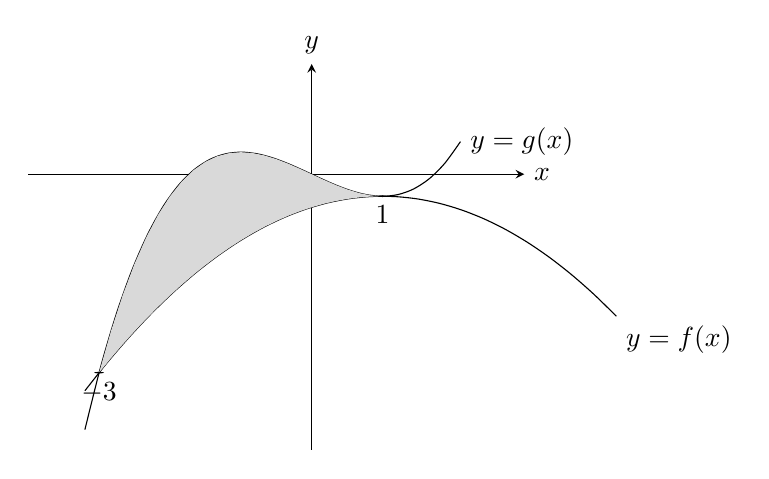
\begin{tikzpicture}[xscale=0.9, yscale=0.14, >=stealth]
  \draw[->] (-4,0) -- (3,0) node[right] {$x$};
  \draw[->] (0,-25) -- (0,10) node[above] {$y$};
  \draw[domain=-3.2:2.1, smooth] plot (\x,{\x*\x*\x-3*\x}) node[right] {$y=g(x)$};
  \draw[domain=-3.2:4.3, smooth] plot (\x,{-(\x-1)*(\x-1)-2}) node[below right] {$y=f(x)$};
  \fill[gray!30, domain=-3:1, variable=\x] plot ({\x},{\x*\x*\x-3*\x}) -- plot[domain=1:-3] ({\x},{-(\x-1)*(\x-1)-2}) -- cycle;
  \fill (-3,-18) circle (2pt) node[below] {$-3$};
  \fill (1,-2) circle (2pt) node[below] {$1$};
\end{tikzpicture}
\end{center}

もとめる面積$S$として
\[
S=\int_{-3}^1(g(x)-f(x))dx=\int_{-3}^1(x-1)^2(x+3)dx=\frac{1}{12}\cdot4^4=\frac{64}{3}
\]
\end{proof}

\newpage

\section*{第5問}

\begin{proof}[解]
\[
A(m,n)=\int_0^1\left(1-x^{\frac1m}\right)^ndx \quad\cdots\text{①}
\]

\textbf{(1)} ①で$(m,n)=(m,1)$として
\[
A(m,1)=\int_0^1\left(1-x^{\frac1m}\right)dx=\left[x-\frac{1}{1+\frac1m}x^{\frac1m+1}\right]_0^1=\frac{1}{m+1}
\]

\textbf{(2)}
\[
A(m,n+1)=\int_0^1\left(1-x^{\frac1m}\right)^{n+1}dx, \qquad
A(m+1,n)=\int_0^1\left(1-x^{\frac{1}{m+1}}\right)^ndx
\]
部分積分法から
\[
A(m,n+1)=\left[x\left(1-x^{\frac1m}\right)^{n+1}\right]_0^1+\int_0^1(n+1)x\left(1-x^{\frac1m}\right)^n\frac1mx^{\frac1m-1}dx
\]
\[
=\frac{n+1}{m}\int_0^1x^{\frac1m}\left(1-x^{\frac1m}\right)^ndx
\]
$p=x^{\frac{m+1}{m}}$とおくと，$\dfrac{dp}{dx}=\dfrac{m+1}{m}x^{\frac1m}$，$x:0\to1$で$p:0\to1$だから，
\[
A(m,n+1)=\frac{n+1}{m}\int_0^1\frac{m}{m+1}\left(1-p^{\frac{1}{m+1}}\right)^ndp=\frac{n+1}{m+1}\int_0^1\left(1-x^{\frac{1}{m+1}}\right)^ndx=\frac{n+1}{m+1}A(m+1,n)
\]

\textbf{(3)} (2)をくり返し用いて，(1)より
\[
A(m,n)=\frac{n(n-1)\cdots2}{(m+1)(m+2)\cdots(m+n-1)}A(m+n-1,1)=\frac{n!m!}{(m+n-1)!}\cdot\frac{1}{m+n}=\frac{n!m!}{(m+n)!}
\]
\end{proof}

\end{document}
